\documentclass[11pt]{asaproc}
\pagestyle{empty}
\usepackage{hyperref}
\usepackage{harvard}
\usepackage{amsthm,amsfonts,amsmath}
\usepackage{enumitem}
%\usepackage[pdftex]{graphicx}%%for Pdftex
\usepackage{graphicx}%%for Latex
\usepackage{multirow}
\usepackage{bbm}
\usepackage{amssymb}
\usepackage{amsthm}
\usepackage{url}
\usepackage{mathrsfs}
\usepackage{appendix}
%\usepackage[pdftex]{graphicx}
%\usepackage{subfigure}
%\usepackage{multicol}
%\usepackage{color}
\usepackage{algorithm}
\usepackage{algorithmic}
\usepackage{setspace}

%set dimensions of columns, gap between columns, and paragraph indent 
%\setlength{\textheight}{8.5in}
%\setlength{\textwidth}{5in}
%\setlength{\headheight}{0cm}
%\setlength{\headsep}{0cm}
%%\setlength{\footheight}{0.0in}
%\setlength{\parindent}{1pc}

%macro
%%%%%%%%%%%%%%%%%%%%%%%%%%%%%%%%%%%%%%%%%%%%%%%%%%%%%%%%%%%%%%%%%%%%%%%%%
\hyphenation{con-tin-u-ous-time con-tin-u-ous bank-rupt-cy}
\hyphenation{Lebes-gue} \hyphenation{ter-mi-nol-o-gy}
%%%%%%%%%%%%%%%%%%%%%%%%%%%%%%%%%%%%%%%%%%%%%%%%%%%%%%%%%%%%%%%%%%%%%%%%%
\newcommand{\bbr}{\mathbb{R}}  %black board bold \mathbb{R}
\newcommand{\bbn}{\mathbb{N}}
\newcommand{\bbp}{\mathbb{P}}
\newcommand{\bY}{\mathbf{Y}}
\newcommand{\mun}{\lceil \mu n \rceil}
\newcommand{\etan}{\lceil \eta n \rceil}
\newcommand{\bbq}{\mathbb{Q}}
\newcommand{\wQ}{\widetilde{\bbp}}%change per Prof. Lai's request to alleviate confusion
\newcommand{\wq}{\widetilde{p}}%change per Prof. Lai's request to alleviate confusion
\newcommand{\wY}{\widetilde{Y}}
\newcommand{\wX}{\widetilde{X}}
\newcommand{\ow}{\overline{w}}
\newcommand{\wht}{\widehat}
\newcommand{\var}{\ensuremath{\mathbb Var}}
\newcommand{\wbY}{\widetilde{\bY}}
\newcommand{\abs}[1]{\lvert#1\rvert}
\newcommand{\D}{\mathbb{D}}
\newcommand{\G}{\mathbb{G}}
\newcommand{\bbe}{\mathbb{E}}
\newcommand{\F}{\mathbb{F}}
\newcommand{\HH}{\mathbb{H}}
\newcommand{\bbj}{\mathbb{J}}
\newcommand{\bbz}{\mathbb{Z}}
\newcommand{\bbs}{\mathbb{S}}
\newcommand{\C}{\mathbb{C}}
\newcommand{\bu}{\mathbf{u}}
\newcommand{\bx}{\mathbf{x}}
\newcommand{\fn}{\footnote}
\newcommand{\ci}{\citeasnoun}
\newcommand{\om}{\omega}
\newcommand{\la}{\lambda}
\newcommand{\tla}{\tilde{\lambda}}
\newcommand{\doth}{f}
\renewcommand{\labelenumi}{\roman{enumi}}
\newcommand{\ps}{P}
\newcommand{\pss}{\ensuremath{\mathbf{p}}} %small boldface
\newcommand{\pmq}{\ensuremath{\mathbf{Q}}}
\newcommand{\pmqs}{\ensuremath{\mathbf{q}}}
\newcommand{\pas}{P-a.s. }
\newcommand{\pasm}{P\mbox{-a.s. }}
\newcommand{\asm}{\quad\mbox{a.s. }}
\newcommand{\cadlag}{c\`adl\`ag }
\newcommand{\fil}{\mathcal{F}}
\newcommand{\gcal}{\mathcal{G}}
\newcommand{\hcal}{\mathcal{H}}
\newcommand{\jcal}{\mathcal{J}}
\newcommand{\pcal}{\mathcal{P}}
\newcommand{\ecal}{\mathcal{E}}
\newcommand{\bcal}{\mathcal{B}}
\newcommand{\ical}{\mathcal{I}}
\newcommand{\scal}{\mathcal{S}}
\newcommand{\ncal}{\mathcal{N}}
\newcommand{\lcal}{\mathcal{L}}
\newcommand{\kcal}{\mathcal{K}}
\newcommand{\acal}{\mathcal{A}}
\newcommand{\mcal}{\mathcal{M}}
\newcommand{\rcal}{\mathcal{R}}
\newcommand{\tcal}{\mathcal{T}}
\newcommand{\ti}{\times}
\newcommand{\we}{\wedge}
\newcommand{\be}{\begin{equation}}
\newcommand{\ee}{\end{equation}}
\newcommand{\bew}{\begin{equation*}}
\newcommand{\eew}{\end{equation*}}
\newcommand{\uK}{\underline K}
\newcommand{\oK}{\overline K}
\renewcommand{\th}{\tilde{h}}
\newcommand{\imp}{\eta}
\newcommand{\xbar}{\overline{X}}
\newcommand{\Xij}{X_{i,j}}
\newcommand{\f}{\left}
\newcommand{\g}{\right}
\newcommand{\naiveest}{\wht{\sigma^2_n}}
\newcommand{\deltaest}{\wht{\sigma^2_d}}

%theorem style
\newtheorem{thm}{Theorem}
\newtheorem{cond}[thm]{Condition}
\newtheorem{defi}[thm]{Definition}
\newtheorem{algo}[thm]{Algorithm}
\newtheorem{prop}[thm]{Proposition}
\newtheorem{corollary}[thm]{Corollary}
\newtheorem{lem}[thm]{Lemma}
\newtheorem{rem}[thm]{Remark}
\newtheorem{ex}[thm]{Example}
\newtheorem{ass}[thm]{Assumption}

\begin{document}

%don't want date printed
\date{}

%make title bold and 14 pt font (Latex default is non-bold, 16pt) 
\title{\Large\bf Choice of the Randomization Unit in Online Controlled Experiment}

%for single author (just remove % characters)
%\author{Shaojie Deng \\
%  Microsoft \\
%  Redmond, WA, 98052}

%for two authors (this is what is printed)
%\author{
%\begin{tabular}[t]{c@{\extracolsep{8em}}c}
%Shaojie Deng  &  Roger Longbotham & Toby Walker & Ya Xu  \\
%  Microsoft & Microsoft & Microsoft & Microsoft 
%% alexdeng@microsoft.com & roger.longbotham@microsoft.com & toby.walker@microsoft.com & yaxu@microsoft.com 
%\end{tabular}
%}
\author{Shaojie Deng\footnote{Microsoft, Redmond, WA 98052, USA, email: {\tt alexdeng@microsoft.com}.}\;\;\;\; Roger Longbotham\footnote{Microsoft, Redmond, WA 98052, USA, email: {\tt roger.longbotham@microsoft.com}.}\;\;\;\; Toby Walker\footnote{Microsoft, Redmond, WA 98052, USA, email: {\tt toby.walker@microsoft.com}.}\;\;\;\; Ya Xu\footnote{Microsoft, Redmond, WA 98052, USA, email: {\tt yaxu@microsoft.com}.} } \normalsize

\date{ \today}
\maketitle

%So first page doesn't have a page number
\thispagestyle{empty}

\subsection*{Abstract}
Controlled experiment has been used widely to support data driven decision making for on-line businesses. By applying appropriate randomization of the experiment units, causal inference can be established. The choice of the experiment unit for randomization can vary. User and page view are two mostly used units. Moreover, the analysis unit is sometimes different from the experiment unit. There are pros and cons in choosing which experiment unit to use and the choice affects the downstream statistical analysis. Generally for page level metrics, randomization by page will have an edge in power due to variance reduction. In this paper, we compare the two experiment units and provide a method to correctly analyze a page view randomization experiment in a two layer randomization framework.
     
\subsection*{Keywords}
Controlled experiment, Experimentation, A/B testing, randomization unit, Variance estimation. 


\section{Introduction}\label{intro}
For centuries people have been looking for ways to evaluate ideas. Controlled experiment, also called randomization test or A/B test has long established its importance as the methodology to establish a causal relationship. This paper will be focused on controlled experiment on the web. An obvious difference controlled experiment on the web and other types of controlled experiment (for example, clinical trials) is that it is easy and also with low cost to collect data on web. In other words, web provides an unprecedented opportunity for us to use the power of controlled experiment to test and evaluate ideas quickly. It is our strong belief that unlock the huge data on the web and use the right methodology to analyze it is the key toward a data driven philosophy, and controlled experiment has successfully set a standard in the industry.  There are already many publications in the literature on controlled experiment. For a good and thorough survey on how to run web experiments, see \ci{expsurvey}.  Most of the works in the literature are focused on practical issues and best practices. To the author's knowledge few of them have been contributed on the underlying statistical methods. Part of the reason is that the related statistical method --- the widely used two sample t-test are so well known, under i.i.d assumptions. In this paper, we focus on the randomization step itself, and show how to analyze a randomized experiment where page view is used to randomize traffic. 


We will be consistently using the following notations and assumptions through out this paper. Let $n$ be the total number of unique users. Let $X_{i,j}$ be the per-page measurement (e.g. number of clicks on the page) on user $i$'s $j^{th}$ page view and $X_{i,j}$ has mean $\mu_i$ and variance $\sigma_i^2$.  Denote $K_i$ the total number of page views from user $i$ and $N = \sum_{i=1}^n K_i$ be the total number of page views. We assume for any $i$, $X_{i,j},j=1,\dots,K_i$ are i.i.d. and uniformly bounded above by some finite constant.  In particular, we allow $(\mu_i,\sigma_i^2)$ to differ from user to user. We also assume $K_i,i=1,\dots,n$ are i.i.d. and independent of $(\mu_i,\sigma_i^2),i=1,\dots,n$. This last assumption is for the purpose of theoretical investigation and need to be checked case by case in practice. We have checked this assumption for some key metrics of web experiments using empirical data and this assumption is reasonable. In a randomized experiment, we call the unit on which randomization is performed the randomization unit. In analysis phase, a metric will be naturally associated with an unit, which we call it analysis unit. For instance, a user level metric such as clicks per user is associated with user as the analysis unit while page view level metrics such as click through rate is associated with page view. 

The following paper is organized as follows. In Section \ref{user}, we first briefly review the case where user is used as the randomization unit. In particular we are interested in page view level metrics and show how delta method should be used. We also give a formula for the bias introduced should we fail to use delta method. In Section \ref{page}, we shift the gear to the case that the randomization unit is page view. We present an asymptotically consistent variance formula of page view level metrics under a two layer randomization framework where a group of users are first recruited and then their page views are randomized into treatment and control. Section \ref{empirical} presents simulation results. In Section \ref{compare}, we discuss the pros and cons of using page view as randomization unit. We suggested extensions and concludes. 


\section{User as Randomization Unit}\label{user}
In this section we focus on the case where the randomization unit is user. In practice users are identified with their login ids or simply cookies stored by the browser. A detailed discussion of user tracking is far beyond the scope of this paper. For this paper, we assume user can be identified perfectly. 

Traditional applications of user randomized experiment is to study movement of user level metrics. From a statistical perspective, this is a vanilla application of two sample t-test to test the null hypothesis that treatment group and control group are the same under the i.i.d assumption. To be more specific, a user level metric is a sample mean of user level measurements. Since users are randomized into control and treatment group, it is safe to assume user level measurements are independent and identically distributed. Under the hierarchical model in Section \ref{intro}, this means we draw $(\mu_i, \sigma_i^2)$ independently for each user and then user level measurements for that particular user is drawn from corresponding distribution. Denote the user level metrics in control and treatment by $\wX_T$ and $\wX_C$, it is clear that they are independent. By central limit theorem,  
\begin{align}\label{zstat}
\frac{\wX_T - \wX_C}{\sqrt{\var \{\wX_T - \wX_C\}}} \to Z,
\end{align}
where $Z$ is standard normal. The two sample t-test is to replace $\var \{\wX_T - \wX_C\}$ by its estimate. In this particular case since $\wX_T$ and $\wX_C$ independent, $\var \{\wX_T - \wX_C\}= \var \wX_T + \var \wX_C$ and both terms in the right hand side can be simply estimated via sample variances. Also, for web experiment, $n$ is large (much much larger than most applications of two sample t-test). Therefore we might as well treat t-statistics as standard normal. 

For page view level metrics, \eqref{zstat} still holds when $\wX_T$ and $\wX_C$ are replaced by page view level metrics $\xbar_T$ and $\xbar_C$. However, $\var \{\xbar_T - \xbar_C\}$ can not be estimated by sample variances. Delta method is needed for variance estimation of $\var \xbar_g$, $g=T,C$; see Section \ref{user-page}. Moreover, when randomization unit is not user, $\xbar_T$ and $\xbar_C$ are not even independent and we need to estimate $\var \{\xbar_T - \xbar_C\}$ directly. This will be our topic in Section \ref{page}. 

\subsection{Page Level Metrics and Delta Method}\label{user-page}
Under our hierarchical model introduced in Section \ref{intro}, a page level metric can be denoted by:
\begin{align*}
\xbar= \frac{\sum_{i=1}^n\sum_{j=1}^{K_i} X_{i,j}}{N}.
\end{align*}
When user is the randomization unit, $\xbar_T$ and $\xbar_C$ are independent and $\var \{\xbar_T-\xbar_C\} = \var \xbar_T + \var \xbar_C$. Therefore we only need to focus on estimating $\var \xbar$. To this end, it is tempting to treat page level metrics $X_{i,j}$, $j=1,\dots,K_i$, $i=1,\dots,n$, as i.i.d. and $\xbar$ under this assumption is an average of i.i.d. samples so the variance of $\xbar$ can be easily estimated by
\begin{align*}
\frac{1}{N^2} \Bigl (\sum_{i=1}^n \sum_{j=1}^{K_i} (X_{i,j}-\overline{X})^2 \Bigr ).
\end{align*}
This estimator, which we call the \emph{naive} estimator,  is not consistent because in our model the user effect $(\mu_i,\sigma_i^2)$ are also a random sample from a distribution and page view level measurements $X_{i,j}$ of the same user are only independent conditioned on $(\mu_i,\sigma_i^2)$. Nevertheless, it is true in our model that the user level measurement $(\sum_{i=1}^{K_i} X_{i,j}, K_i),i=1,\dots,n$ are i.i.d. By letting $Y_i = \sum_{i=1}^{K_i} X_{i,j}$ and express $\xbar$ as $\sum_{i=1}^n Y_i / \sum_{i=1}^n K_i$, it is then a straightforward application of the delta method to get an asymptotically consistent estimator for $\var \xbar$:
\begin{align*}
\frac{1}{n} \Bigl\{ \frac{1}{\wht{\bbe K_i}^2}\wht{\var Y_i} + \frac{\wht{\bbe Y_i}^2}{\wht{\bbe K_i}^4}\wht{\var K_i} - 2\frac{\wht{\bbe Y_i}}{\wht{\bbe K_i}^3} \wht{Cov(Y_i,K_i)} \Bigr\} 
\end{align*}
where these ``hatted'' quantities are the sample mean, variance or covariance. 

For asymptotic analysis, we will let $n\to \infty$ (so $N\to \infty$ a.s.). To normalize the naive estimator and delta method estimator, we multiply them by $n$ so that they will converge to some nonzero numbers.  We introduce the normalized naive estimator 
\begin{align}
\wht{\sigma^2_n} = n\frac{1}{N^2} \Bigl (\sum_{i=1}^n \sum_{j=1}^{K_i} (X_{i,j}-\overline{X})^2 \Bigr )
\end{align}
and the normalized delta method estimator
\begin{align}
\wht{\sigma^2_d} = \frac{1}{\wht{\bbe K_i}^2}\wht{\var Y_i} + \frac{\wht{\bbe Y_i}^2}{\wht{\bbe K_i}^4}\wht{\var K_i} - 2\frac{\wht{\bbe Y_i}}{\wht{\bbe K_i}^3} \wht{Cov(Y_i,K_i)}.
\end{align}


A natural question to ask is how biased is the naive estimator $\naiveest$ relative to the true normalized variance $n\var \xbar$. This is answered in the following theorem.
\begin{thm}\label{thm1.1}
Let $C = \frac{\bbe K_i^2}{(\bbe K_i)^2}$.  Then, as $n\to \infty$,
\begin{align}
n\var\xbar &\to C \var(\mu_i) + \bbe(\sigma^2_i)/\bbe (K_i)\label{truevar} \\
\deltaest & \to  C \var(\mu_i) + \bbe(\sigma^2_i)/\bbe (K_i)\label{deltalim}  \\
\naiveest & \to  \frac{1}{\bbe(K_i)} (\var(\mu_i)+\bbe(\sigma_i^2))\label{naivelim}.
\end{align}
Let $\rho:= \var(\mu_i)/(\var(\mu_i)+\bbe(\sigma^2_i))$ be the user effect coefficient(variances that explained by between user variation), then
\begin{align}
\frac{n\var (\xbar)}{\naiveest} \to  (\bbe(K_i)C - 1)\rho +1.
\end{align}
The convergence in \eqref{deltalim} and \eqref{naivelim} are  in probability. 
\end{thm}

\begin{proof}[Proof of Theorem \ref{thm1.1}.]
\eqref{deltalim} follows directly from the property of the delta method. To prove \eqref{truevar}, we first apply conditional variance formula by conditioning on $(\mu_i,\sigma_i^2, K_i,\newline i=1,\dots,n)$. This gives
\begin{align*}
&\var \xbar =  \var  \Bigl( \bbe\Bigl(   \frac{\sum_{i=1}^n\sum_{j=1}^{K_i} X_{i,j}}{N} \Big| K_i,\mu_i,\sigma_i^2,  i=1,\dots,n\Bigr) \Bigr) \\
+&\bbe \Bigl(\var \Bigl( \frac{\sum_{i=1}^n\sum_{j=1}^{K_i} X_{i,j}}{N} \Big | K_i,\mu_i,\sigma_i^2,  i=1,\dots,n\Bigr)\Bigr) \notag\\
=&\var \Bigl(\frac{1}{N}\sum_{i=1}^n K_i \mu_i \Bigr)+\bbe \Bigl(\frac{1}{N^2}\sum_{i=1}^n K_i \sigma^2_i \Bigr).
\end{align*}
Let  $w_i = K_i/\sum_{i=1}^n K_i = K_i/N$. Since $K_i$ independent of $(\mu_i, \sigma^2_i)$ and $N/n \to \bbe {K_i}$ as $n\to \infty$, we can further simplify the right hand. First, by applying iterative expectation(frist conditioning on $w_1,\dots, w_n$), we have  
\begin{align}
n \bbe \Bigl(\frac{1}{N^2}\sum_{i=1}^n K_i \sigma^2_i \Bigr)  = \sum_{i=1}^n \bbe\Bigl( \frac{n}{N} w_i\sigma^2_i \Bigr) = \frac{1}{\bbe K_i}(\sum_{i=1}^n w_i)\bbe \sigma_i^2 = \frac{\bbe \sigma_i^2}{\bbe K_i} \label{withinterm}
\end{align}
where the second equality is by bounded convergence theorem(since $N/n \to \bbe {K_i}$ and $\sum w_i\sigma^2_i$ bounded) and the last equation is from $\sum w_i=1$. Since $(\mu_i, \sigma^2_i)$ are i.i.d., 
\begin{align}
&n\var (\sum_{i=1}^n w_i \mu_i) = n\bbe (\var (\sum_{i=1}^n w_i \mu_i|w_1,\dots,w_n))+ n\var (\bbe (\sum_{i=1}^n w_i \mu_i|w_1,\dots,w_n)) \\
&=  n\bbe (\sum_{i=1}^n w_i^2 \var(\mu_i)) + n \var((\sum_{i=1}^n w_i)\bbe\mu_i ) = n\bbe(\sum_{i=1}^n w_i^2) \var (\mu_i) \label {betweenterm}
\end{align}
where the last equality is from the fact that the second term is $0$. By simple algebra, 
$n \sum_{i=1}^n w_i^2 =  \frac{\overline{K_i^2}}{\overline{K_i} \times \overline{K_i}}$, where $\overline{K_i^2}$ and $\overline{K_i}$ are sample mean of $K_i^2$ and $K_i$, respectively.
By strong law of large number, $\overline{K_i^2}\to \bbe K_i^2$ a.s., $\overline{K_i}\to \bbe K_i$ a.s., therefore $n \sum_{i=1}^n w_i^2 \to  \frac{\bbe{K_i^2}}{(\bbe{K_i})^2}$ a.s. Combine this result with \eqref{withinterm} and \eqref{betweenterm}, we've proved \eqref{truevar}.

We now turn to the limit of $\naiveest$. 
\begin{align*}
 \naiveest &= n \frac{1}{N^2} \Bigl (\sum_{i=1}^n \sum_{j=1}^{K_i} (X_{i,j}-\overline{X})^2 \Bigr )= \frac{n}{N^2} \Bigl \{  \sum_{i=1}^n \sum_{j=1}^{K_i} X_{i,j}^2 - N \xbar^2 \Bigr\}\\
&\to   \lim_{n\to \infty} \Bigl(\frac{n^2}{N^2}\Bigr) \bbe \bigl(\sum_{j=1}^{K_i} \Xij^2 \bigr) -   \lim_{n\to \infty} \Bigl(\frac{n}{N}\Bigr) (\bbe \mu_i)^2 .
\end{align*}
The last limit is from $(1/n) \sum_{j=1}^{K_i} X_{i,j}^2 \to \bbe \bigl(\sum_{j=1}^{K_i} \Xij^2 \bigr)$ and $\xbar \to \bbe \mu_i$ a.s., both by the strong law of large number.
By $N/n \to \bbe K_i$, and also $\bbe \bigl(\sum_{j=1}^{K_i} \Xij^2 \bigr)  = \bbe K_i \bbe X_{i,j}^2 = \bbe K_i (\bbe \mu_i^2 + \bbe \sigma_i^2)$,
\eqref{naivelim} follows.
\end{proof}


\eqref{truevar} in Theorem \ref{thm1.1} shows the variance of a page level metrics can be decomposed into two parts. The first part $C\var\mu_i$ is contributed by user effect $(\mu_i,\sigma_i^2)$. We call this between user variance. The second part $\bbe(\sigma_i^2)/\bbe(K_i)$ represents the variance not explained by user effect and we might call this within user variance. When $\bbe K_i$ large, note that $C = \bbe K_i^2 / (\bbe K_i)^2 \ge 1$ by Jensen's inequality, the between user variance will dominate. This is intuitively easy to understand since within user variance decrease to $0$ as each user has more and more page views. 

In empirical data, we do see between user variance contributed a large proportion of the total variance, especially for those experiments ran for a few weeks. 
This observation motivated us to use page view as randomization unit for some experiments if the key metrics we are interested in are at page view level. A caveat here is that not all experiment can be done with page view level randomization, mainly due to the inconsistent user experience. We leave the discussion later in Section \ref{compare} and only focus on theoretical property in the next section. 

\section{Page View as Randomization Unit}\label{page}


\subsection{A Two Layer Randomization Framework}
Suppose all page views are randomly divided into different groups. By all page views we mean page views from all users that could show up. Under this framework, it is from the typical marginalization argument that we can treat page view level measurement as i.i.d. i.e., there is no user effect in the analysis because the page views are drawn from all users and no user selection variance is induced in this randomization scheme. Since page view level measurements are i.i.d.,  statistical analysis for page view level metrics is therefore straightforward. 

The case that is of most interest is the following. We first randomly selected $n$ user from all the users that could show up. $n$ is usually only a small percentage of the total number $M$ of users that could show up in the universe. Let us assume $M$ is infinity and hence assume users are drawn independently. All page views from these $n$ users are then randomly split into control and treatment. The goal is to make inference by comparing certain metrics in control and treatment. There are at least two reasons that we favor this two layer randomization framework over the one layer framework mentioned in the previous paragraph. One is that we want to run more than one experiments simultaneously and for a particular page view randomization experiment we only allow part of the whole traffic and reserve other traffic for user randomization experiment. Another reason is that we might not want all users to experience the page level randomization experience, which could potentially be inconsistent or non-sticky. Section \ref{compare} covers this in more detail. 

An obvious difference between page view randomization and user randomization is the availability of many user level metrics. If the randomization unit is page view, first of all, page views per unique user does not make any sense anymore. Other metrics that are often used in search experimentation that will be unavailable include sessions per unique user, queries per unique user, page loading time per unique users, etc. However, as we will see in Section \ref{page-page}, the strength of using page view as randomization unit is the improvement in variance reduction for page level metrics, hence a boost in statistical power.

\subsection{Page Level Metrics}\label{page-page}
Denote a page view level metric as $\xbar_r = \sum_{i=1}^n \sum_{j=1}^{{K_i}^{(r)}}X_{i,j}^{(r)}/N_r$ where $r=1,2$ stands for control and treatment. In Section \ref{user} , we never considered the variance of both control and treatment together. This is because the control and treatment groups have different users and since randomization is based on user, the metrics of the two groups are naturally independent. As a result the variance of the difference of the metrics is simply the sum of the two variances of the same metric in each group.  What make things more complicated here is that under the two layer randomization framework, control and treatment share the same group of $n$ users. It is now the page view, not the user that is randomized into two groups. Due to this very fact, $\xbar_1$ and $\xbar_2$ are no longer independent. 


What we need is an asymptotically unbiased estimator for $\var (\xbar_1-\xbar_2)$ when the page views are split into control and treatment with fixed weights. Under the same hierarchical model, conditioned on $K_i$, $K_i^{(r)}$ follows $binomial(K_i, p)$ distribution where $p$ depends on the weights of treatment and control. If we only consider one group, say control. Then the only difference between this framework and that of Section \ref{user} is that now $K_i^{(r)}$ follows from a different distribution(from $K_i$). But note that all the results in Section \ref{user} does not depend on the distribution of $K_i$. Therefore all results in Section \ref{user} directly apply on $\xbar_1$ (or $\xbar_2$). Particularly,we have the following proposition for free.

\begin{prop}\label{p_prop1}
Let $w_i^{(r)}=K_i^{(r)}/\sum_{i=1}^{n} K_i^{(r)} $ and $C_r =\frac{\bbe (K_i^{(r)})^2}{(\bbe K_i^{(r)})^2}$. Then for $r=1,2$
\begin{align}
\naiveest_r &\to  \frac{1}{\bbe(K_i^{(r)})} (\var(\mu_i)+\bbe(\sigma_i^2)) \label{p_naive}\\
\deltaest_r &\to C_r \var(\mu_i) + \bbe(\sigma^2_i)/\bbe (K_i^{(r)}) \label{p_delta}.
\end{align}
\end{prop}

What Proposition \ref{p_prop1} says is exactly that if we apply naive formula or delta method formula to one group, we will get asymptotically unbiased estimator for the right hand side of \eqref{p_naive} and \eqref{p_delta}, respectively. 

To analyze $\var (\xbar_1-\xbar_2)$, by applying conditioned variance formula as in the proof of Theorem~\ref{thm1.1},
\begin{align}
&\var (\xbar_1-\xbar_2) = \var \Bigl( \frac{\sum_{i=1}^n\sum_{j=1}^{K_i^{(1)}} X_{i,j}^{(1)}}{N_1} -\frac{\sum_{i=1}^n\sum_{j=1}^{K_i^{(2)}} X_{i,j}^{(2)}}{N_2}\Bigr) \notag \\
 =& \var \Bigl( \bbe \Bigl( \frac{\sum_{i=1}^n\sum_{j=1}^{K_i^{(1)}} X_{i,j}^{(1)}}{N_1} -\frac{\sum_{i=1}^n\sum_{j=1}^{K_i^{(2)}} X_{i,j}^{(2)}}{N_2}|K_i^{(r)}, \mu_i^{(r)},\sigma_i^{(r)},i=1,\dots,n, r=1,2) \Bigr)\Bigr)\notag \\
+&\bbe \Bigl(\var \Bigl( \frac{\sum_{i=1}^n\sum_{j=1}^{K_i^{(1)}} X_{i,j}^{(1)}}{N_1^2} -\frac{\sum_{i=1}^n\sum_{j=1}^{K_i^{(2)}} X_{i,j}^{(2)}}{N_2^2}|K_i^{(r)}, \mu_i^{(r)},\sigma_i^{(r)},i=1,\dots,n, r=1,2\Bigr)\Bigr) \notag\\
=&\var \Bigl(\frac{1}{N_1}\sum_{i=1}^n K_i^{(1)} \mu_i  - \frac{1}{N_2}\sum_{i=1}^n K_i^{(2)} \mu_i\Bigr)+\bbe \Bigl(\frac{1}{N_1^2}\sum_{i=1}^n K_i^{(1)} \sigma^2_i   + \frac{1}{N_2^2}\sum_{i=1}^n K_i^{(2)} \sigma^2_i \Bigr)  \label{basicformula2}
\end{align}

By using the short hand notation $w_i^{(r)}$, we can simplify $n\var (\xbar_1-\xbar_2)  $ into 
\begin{align}
n\var\Bigl( \sum_{i=1}^n (w_i^{(1)}-w_i^{(2)})\mu_i\Bigr) + n\bbe \Bigl( \sum_{i=1}^n (w_i^{(1)}/N_1+w_i^{(2)}/N_2)\sigma_i^2\Bigr).
\end{align}
Comparing to \eqref{withinterm}, we see
\begin{align}
n\bbe \Bigl( \sum_{i=1}^n (w_i^{(1)}/N_1+w_i^{(2)}/N_2)\sigma_i^2\Bigr) \to \frac{\bbe \sigma_i^2}{\bbe K_i^{(1)}}+ \frac{\bbe \sigma_i^2}{\bbe K_i^{(2)}}  \label{p_within}
\end{align}
where the last term is because $K_i^{(1)}$ has the same distribution as $K_i^{(2)}$. 


By using conditional variance formula for another time and following the exact same argument as in \eqref{betweenterm} (replace $w_i$ by $(w_i^{(1)}-w_i^{(2)})$), we have
\begin{align}\label{eqraw}
n\var\Bigl( \sum_{i=1}^n (w_i^{(1)}-w_i^{(2)})\mu_i\Bigr) = n\bbe \bigl( \sum_{i=1}^n (w_i^{(1)}-w_i^{(2)})^2 \var \mu_i\bigr) \notag \\
= \Bigl( n\bbe \bigl (\sum_{i=1}^n (w_i^{(1)})^2\bigr)+ n\bbe \bigl (\sum_{i=1}^n (w_i^{(2)})^2\bigr)-2 n\bbe\bigl( \sum_{i=1}^n w_i^{(1)}w_i^{(2)}\bigr)\Bigl) \var \mu_i.
\end{align}

In the proof of Theorem~\ref{thm1.1}, we proved $n\bbe \bigl (\sum_{i=1}^n w_i^2\bigr)\to \frac{\bbe K_i^2}{(\bbe K_i)^2} = C$. Same argument can be extended to prove the following:

\begin{align*}
&n\bbe \bigl (\sum_{i=1}^n (w_i^{(r)})^2\bigr)\to \frac{\bbe (K_i^{(r)})^2}{(\bbe K_i^{(r)})^2} = C_r, r=1,2\\
&n\bbe \bigl (\sum_{i=1}^n (w_i^{(1)}w_i^{(2)})\bigr)\to \frac{\bbe (K_i^{(1)}K_i^{(2)})}{\bbe K_i^{(1)}\bbe K_i^{(2)}}:= C_x.
\end{align*}

Plugging into \eqref{eqraw} entails
\begin{align}\label{p_between}
n\var\Bigl( \sum_{i=1}^n (w_i^{(1)}-w_i^{(2)})\mu_i\Bigr) \to  (C_1+C_2-2C_x) \var \mu_i.
\end{align}


Combining this with \eqref{p_within}, we have proved the following.
\begin{prop}\label{p_prop2}
Under the framework of this section, let $C_r = \frac{\bbe (K_i^{(r)})^2}{(\bbe K_i^{(r)})^2}$ and $C_x = \frac{\bbe (K_i^{(1)}K_i^{(2)})}{\bbe K_i^{(1)}\bbe K_i^{(2)}}$. As $n\to \infty$,
\begin{align}\label{p_truevar}
n\var(\xbar_1-\xbar_2) \to (C_1+C_2-2C_x) \var \mu_i + \sum_{r=1,2} \frac{\bbe \sigma_i^2}{\bbe K_i^{(r)}}.
\end{align}
\end{prop}

The remaining piece is to figure out what is $C_1+C_2-C_x$.  The next result shows $C_1+C_2- 2C_x = \sum_{r=1,2} \frac{1}{\bbe K_i^{(r)}}$. 
\begin{prop}\label{p_prop3}
Suppose control has weight $p$ and treatment weight $q$. 
\begin{align}\label{pcoeff}
C_1+C_2-2C_x = \frac{1 }{\bbe K_i^{(1)}}+\frac{1}{\bbe K_i^{(2)}}.
\end{align}
Therefore, 
\begin{align}\label{varp}
n\var(\xbar_1-\xbar_2) \to \Bigl(\frac{1 }{\bbe K_i^{(1)}}+\frac{1}{\bbe K_i^{(2)}}\Bigr) \Bigl( \var \mu_i + \bbe \sigma_i^2\Bigr).
\end{align}
\end{prop}

\begin{proof}[Proof of Proposition \ref{p_prop3}]
\eqref{varp} follows from Proposition~\ref{p_prop2} and \eqref{pcoeff}. Here we only prove \eqref{pcoeff}. To see this, note that $K_i = K_i^{(1)}+K_i^{(2)}$ and $K_i^{(1)}$ follows $Binomial(K_i, p)$. 
\begin{align*}
\bbe K_i^{(1)} &= p\bbe K_i\\
\bbe K_i^{(2)} &=q\bbe K_i\\
\bbe \bigl((K_i^{(1)})^2\bigr)& = pq \bbe K_i + p^2 \bbe K_i^2\\
\bbe \bigl((K_i^{(2)})^2\bigr)& = pq \bbe K_i + q^2 \bbe K_i^2\\
\bbe K_i^{(1)}K_i^{(2)}& = p \bbe K_i^2 - pq \bbe K_i - p^2 \bbe K_i^2 = pq \bbe K_i^2 -pq \bbe K_i.
\end{align*}
By definition, 
\begin{align*}
C_1+C_2-2C_x &= \frac{\bbe (K_i^{(1)})^2}{(\bbe K_i^{(1)})^2} + \frac{\bbe (K_i^{(2)})^2}{(\bbe K_i^{(2)})^2} - 2 \frac{ p \bbe K_i^2 - pq \bbe K_i - p^2 \bbe K_i^2 = pq \bbe K_i^2 -pq \bbe K_i}{\bbe K_i^{(1)}\bbe K_i^{(2)}}\\
&= \frac{1}{(\bbe K_i)^2}\Bigl(\frac{1}{p^2 }\bbe \bigl((K_i^{(1)})^2\bigr)+\frac{1}{q^2}\bbe \bigl((K_i^{(2)})^2\bigr) - \frac{2}{pq}\bbe K_i^{(1)}K_i^{(2)} \Bigr)\\
& = (q/p + p/q +2) \frac{1}{\bbe K_i} = (1/p+1/q)\frac{1}{\bbe K_i}.
\end{align*}
On the other hand,
\[
\frac{1 }{\bbe K_i^{(1)}}+\frac{1}{\bbe K_i^{(2)}} = (1/p+1/q)\frac{1}{\bbe K_i}. 
\]
Hence $C_1+C_2-2C_x = \frac{1 }{\bbe K_i^{(1)}}+\frac{1}{\bbe K_i^{(2)}}$. 
\end{proof}

We can now summarize the result in this section into the following theorem.
\begin{thm}\label{p_thm1}
Under the framework of this section, as $n\to\infty$
\begin{align*}
n\var(\xbar_1-\xbar_2) \to \Bigl(\frac{1 }{\bbe K_i^{(1)}}+\frac{1}{\bbe K_i^{(2)}}\Bigr) \Bigl( \var \mu_i + \bbe \sigma_i^2\Bigr).
\end{align*}
Moreover $\naiveest_1+\naiveest_2$ is an asymptotically unbiased estimator for $n\var(\xbar_1-\xbar_2)$.
\end{thm}

In the following of this paper, we denote $\naiveest_1+\naiveest_2$ as Formula P, where P stands for ``randomization by page view''.



\section{Simulation and Empirical Results}\label{empirical}
We use page click rate (PCR) as example to verify Formula P and show how it performs. We also compare the variance of PCR from a randomization by user experiment to that from a page view randomization experiment to empirically see the variance reduction from page view randomization. Like click through rate (CTR), page click rate is a page based metric focusing on users' click engagement on a page. The difference between PCR and CTR is that the page view level measurement of CTR is the total number of clicks on the page for a page view, while for PCR it is a binary number indicating whether a page view generates any click.  
For a fixed $n$, we first simulate $p_i$, $i=1,\dots,n$, the click through rate for a user from a $Beta(0.1,0.5)$ distribution(see Figure~\ref{fig:beta} to get a sense of the shape of the distribution). We then simulate the total number of page view $K_i$ from some distribution, which we can vary, and then use binomial distribution to split $K_i$ into $K_i^{(1)}$ and $K_i^{(2)}$. For user $i$, we then simulate $\sum_{j=1}^{K_i^{(r)}}X_{i,j}^{(r)}$ from $Binomial(p_i)$. 
In each simulation run, we record $\xbar_1-\xbar_2$, as well as  $\naiveest$, $\wht{C_1}$,$\wht{C_2}$, $\wht{C_x}$, $\wht{\bbe K_i^{(r)}}$. \footnote{For $\naiveest$, $\wht{C_1}$, $\wht{C_2}$, $\wht{\bbe K_i^{(r)}}$, we can actually calculate from both control and treatment and then take the average to get a more accurate estimate.} We repeat this step for $1000$ times. After the $1000$ simulation run, we can estimate $\var{(\xbar_1-\xbar_2)}$ from the sample variances of the $1000$ realizations of $\xbar_1-\xbar_2$, which we denote by $\wht{\sigma^2_{sim}}$ for the normalized variances, which is $n$ times the sample variance of $\xbar_1-\xbar_2$. We also use bootstrap simulation(100 subsamples) to get an estimate of the standard deviation of the normalized variance estimator $\wht{\sigma^2_{sim}}$. On the other hand, for each of these $1000$ simulation run, we can apply Formula P to estimate the normalized variance. We then compare the distribution of these $1000$ estimates from Formula P to the 95\% confidence interval $(\wht{\sigma^2_{sim}} - 1.96SD(\wht{\sigma^2_{sim}}), \wht{\sigma^2_{sim}} + 1.96SD(\wht{\sigma^2_{sim}}))$. In all the simulation, we fixed $n=100,000$ and $p=q = 0.5$.

\begin{figure}[!hbtp]
  \centering
  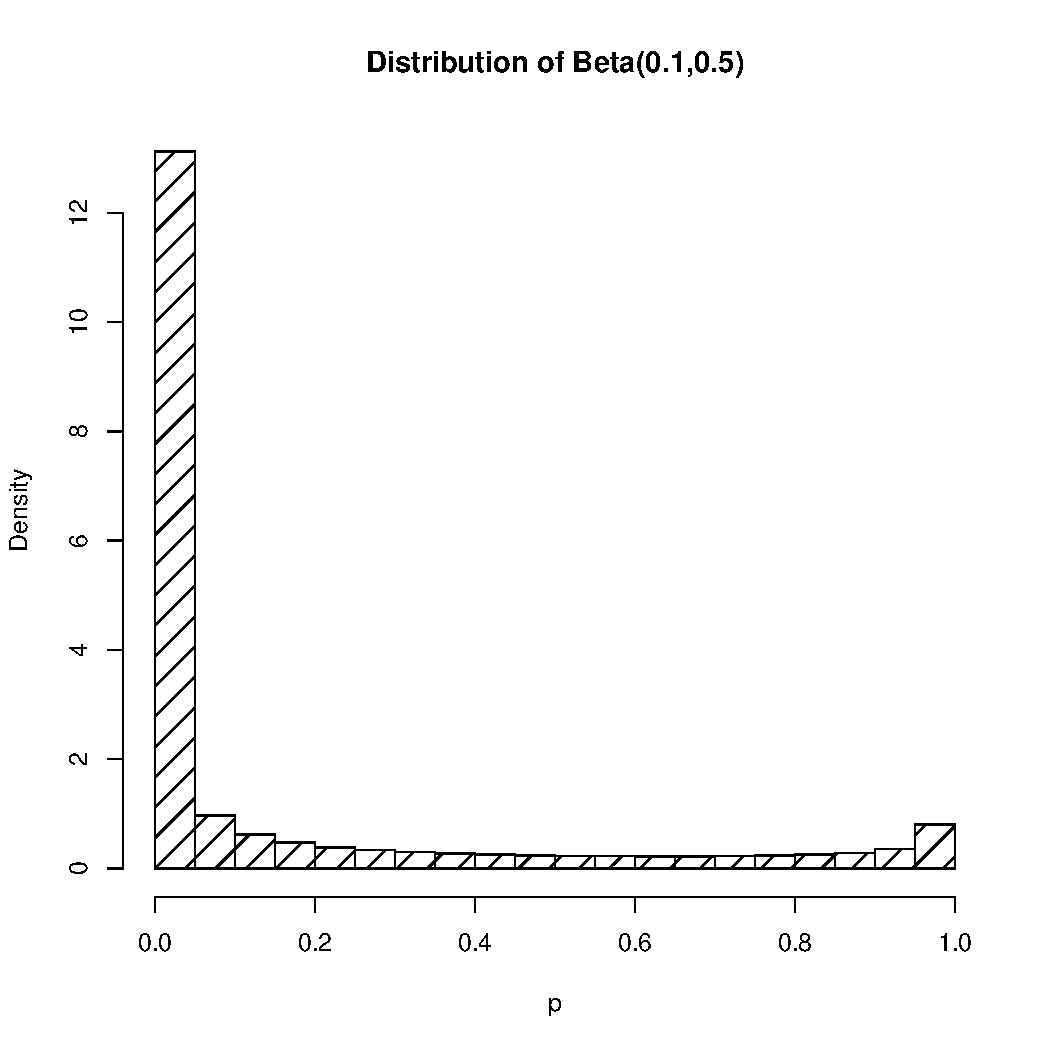
\includegraphics[width=0.5\textwidth]{beta-dist}
  \caption{The histogram of $p_i$ for $n=100,000$ users from a $Beta(0.1,0.5)$ distribution.}
  \label{fig:beta}
\end{figure}

\subsection{Performance of Formula P}
We first use $Poisson(6)$ to generate $K_i$. The plot on the left in Figure \ref{fig:kpois6} shows that $C_1+C_2-2C_x$ is indeed close to $1/\bbe K_i^{(1)}+1/\bbe K_i^{(2)}$. The ratio of the two is normally distributed and concentrated around 1. The plot on the right shows all the $1000$ estimates from Formula P are within the bootstrapped 95\% confidence interval.
\begin{figure}[!hbtp]
  \centering
  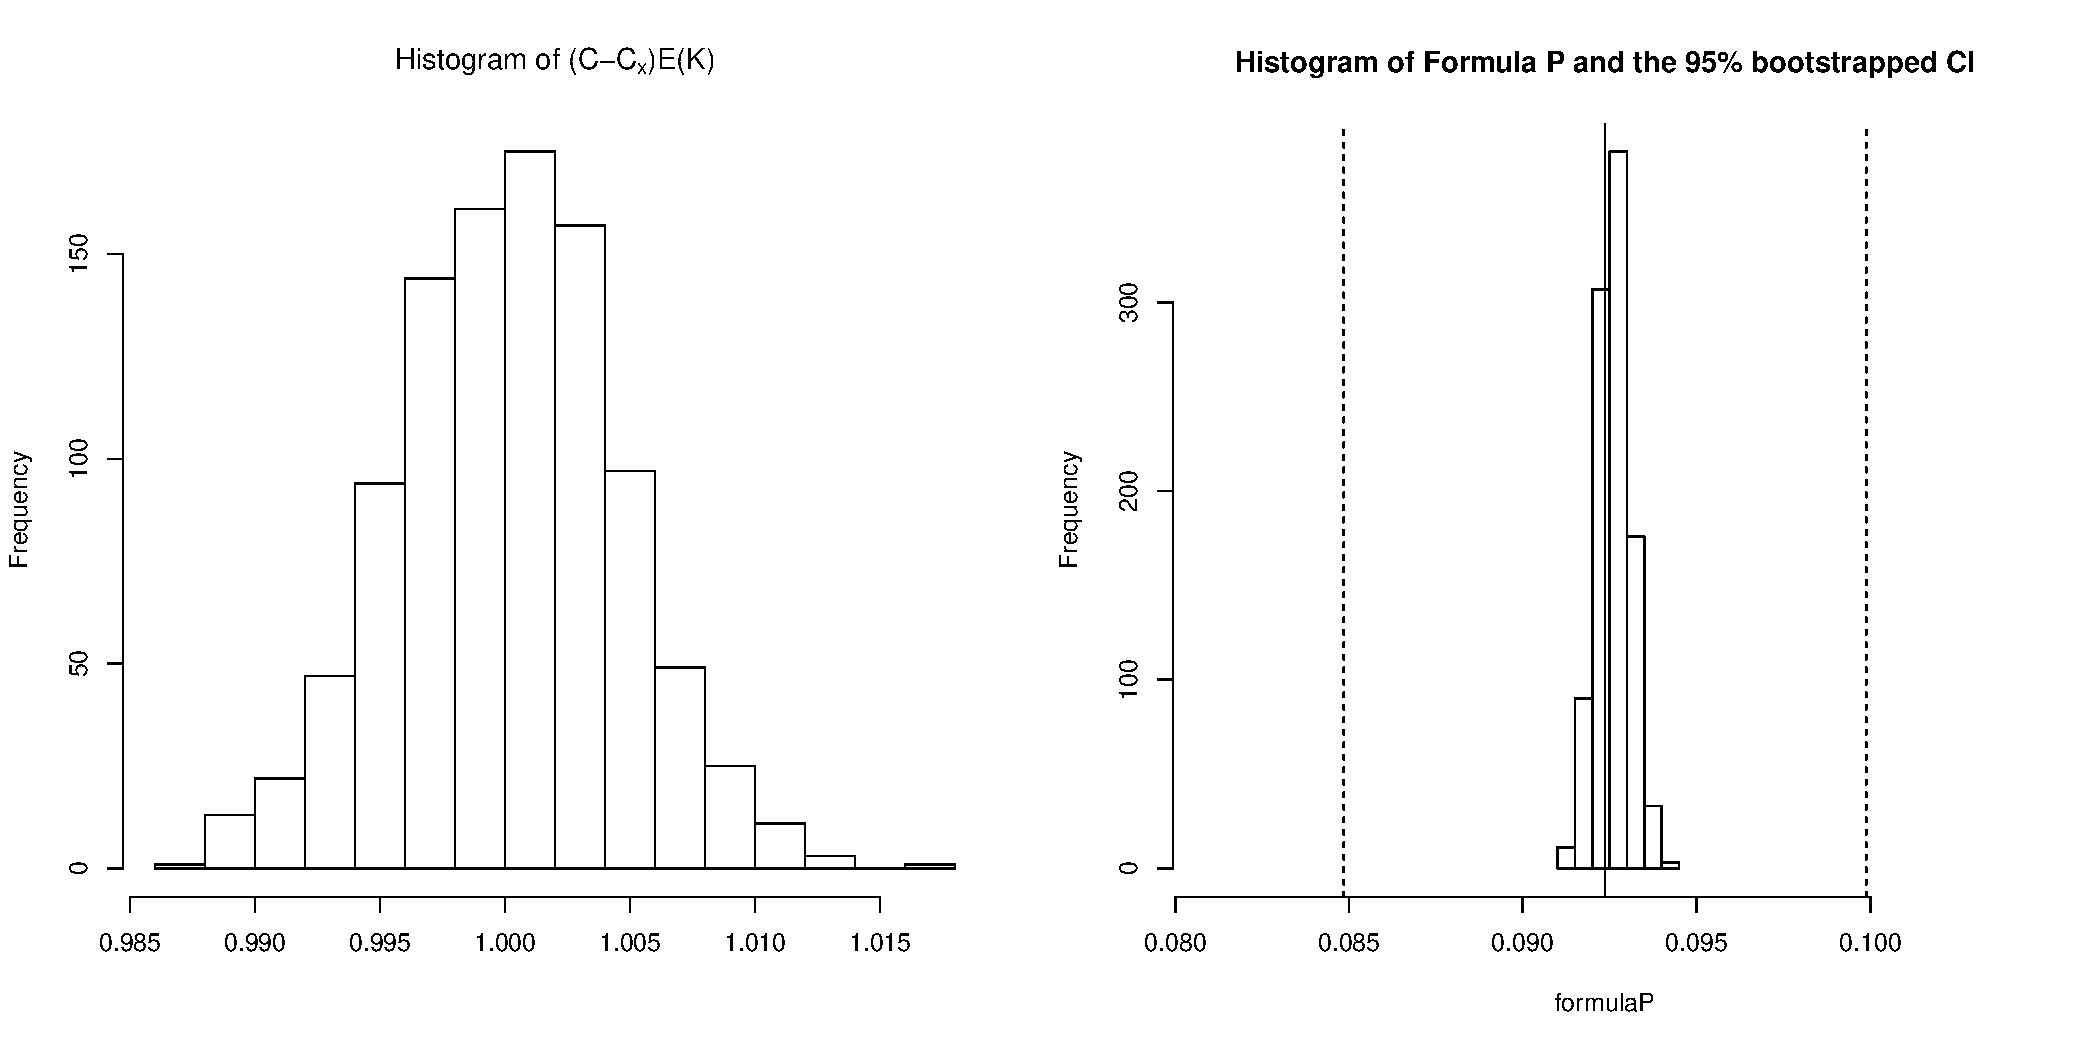
\includegraphics[width=.9\textwidth]{kpois6}
  \caption{$K_i$ from Poisson(6) distribution. Left: Histogram of $(\wht{C1}-\wht{C_x})\wht{\bbe K_i^{(1)}}$. Right: Histogram of the $1000$ estimates from Formula P and the 95\% confidence interval form bootstrap. The two dashed lines are lower and upper bound of the confidence interval and the solid line is the sample variance of $1000$ realization of $\xbar_1-\xbar_2$ multiplied by $n$}
  \label{fig:kpois6}
\end{figure}
\begin{figure}[!htbp]
  \centering
  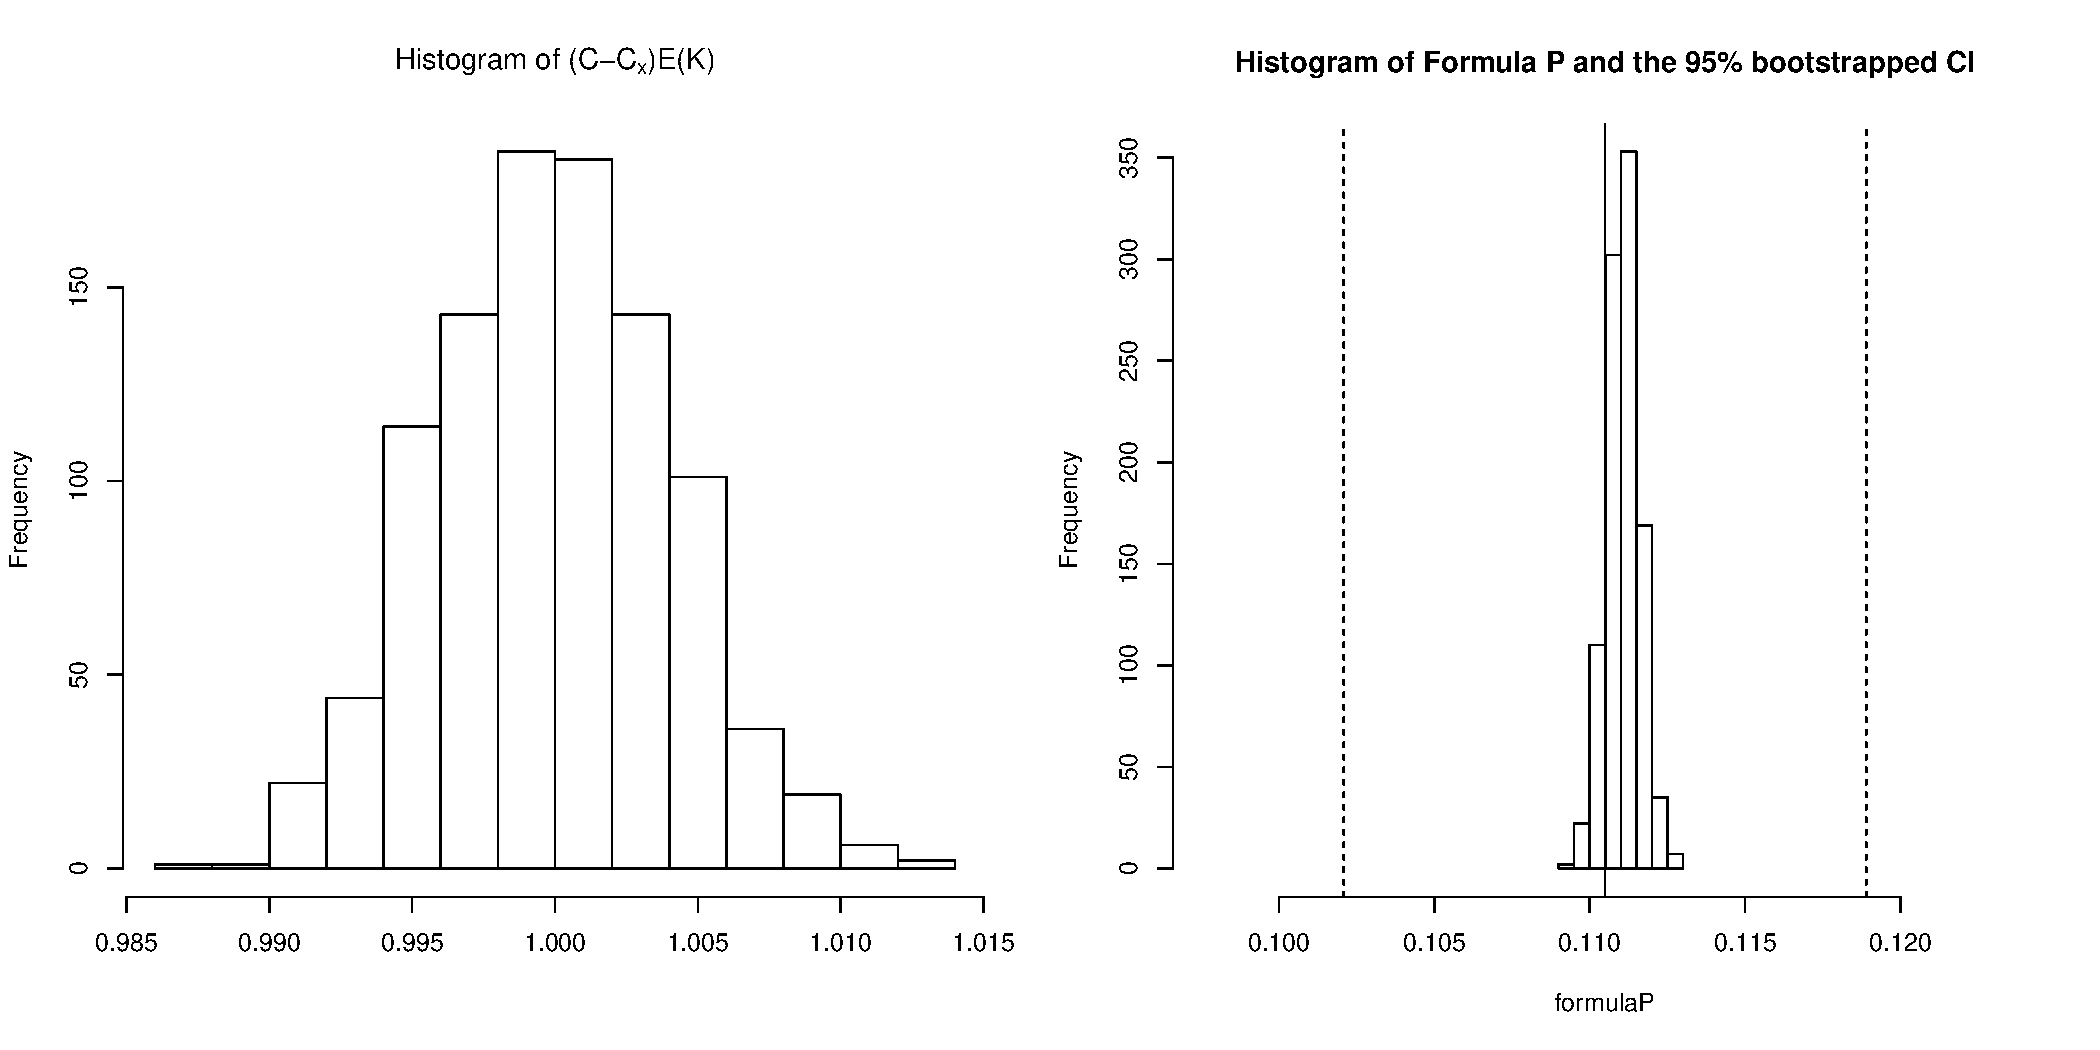
\includegraphics[width=.9\textwidth]{kfixed5}
    \caption{$K_i=5$. Left: Histogram of $(\wht{C_1}-\wht{C_x})\wht{\bbe K_i^{(1)}}$. Right: Histogram of the $1000$ estimates from Formula P and the 95\% confidence interval form bootstrap. The two dashed lines are lower and upper bound of the confidence interval and the solid line is the sample variance of $1000$ realization of $\xbar_1-\xbar_2$ multiplied by $n$}
  \label{fig:kfixed5}
\end{figure}

In Figure~\ref{fig:kfixed5}, we fixed $K_i=5$, $i=1,\dots, n$. The simulation shows similar performance of Formula P.

\subsection{Variance Reduction}
In this simulation study, we compare the variance of PCR from a user randomized experiment with a page view randomized experiment. $p_i$ follows from the same Beta distribution as in the previous section. We simulate $K_i$ in two steps. First, simulate number of sessions of user $i$ from a Poisson(2) distribution, then for each session, simulate number of page views from Poisson(3). $K_i$ for user $i$ is the sum of all page views from all sessions. To simulate a user randomization experiment, $n$ users are then randomized into control and treatment group. To simulate a page view randomized experiment, for each user, $K_i$ page views are randomized into control and treatment groups. For each cases, we run 1000 simulations just as we did in the previous section. Figure \ref{fig:compare} shows the results of user randomization and page view randomization together. We can see that the variances when we randomize by user is around 0.64 while the variance when randomization is on page view is about 0.092. Therefore, there is a variance reduction at a factor of 7!

\begin{figure}[!htbp]
  \centering
  \includegraphics[width=\textwidth]{jsmpreceding_compare}
    \caption{Randomization by user vs. randomization by page view.}
  \label{fig:compare}
\end{figure}


\section{Conclusion}\label{compare}
In this paper, we have provided a way to analyze page view level metrics from an experiment with page view as the randomization unit, under a two layer randomization framework. In particular, we presented a formula for variance estimation and compare the variance from a page view randomized experiment to corresponding user randomized experiment and showed that page view randomized experiment leads to smaller variance for the same page view level metric. 

Aside from theoretical property, in practice the more important topic is how do we choose randomization unit between user and page view. The most apparent distinction between the two is whether the user experience is consistent. If randomization is applied on page view, then by design a same user will receive both control and treatment experience.  This non-sticky experience might be problematic and even a bad experiment design if the change between treatment and control experience is so large that swapping between them will cause huge user confusion. There are also many cases that one expects certain treatment effect that will require a user to receive a consistent experience for a period of time for the effect to show up. Whenever consistent user experience is a must, randomization unit should be no finer than user level. Also, we cannot track any user level metrics if randomize by page view. For example, many loyalty metrics such as number of visits per user is at user level.  Page view level randomization, on the other hand, still provide an intriguing alternative to user level randomization. As we have shown in this paper, it has an advantage in terms of statistical power on page level metrics due to the variance reduction. There are also cases when we want initial data collection for certain features that we do not want user to consistently experience. As an example, one might want to intentionally slowing down the page loading to study how the page abandon rate will change. 

There are a few other alternatives besides user and page. One of them is to randomize by visits. This will guarantee that same user will have consistent experience within each visit, while still gains some variance reduction over pure user randomization by exposing the same user to both treatment and control on different visits. Another choice appeared in the literature was user-day randomization; see \ci{googlesurvey}. We mark the theoretical and empirical investigation of these different randomization units as future work. 



%cite further references
\nocite{googlesurvey} 
\nocite{asympstat}

\bibliography{biblio}
\bibliographystyle{jmr}
\end{document}
